\documentclass[a4paper,titlepage]{article}
\usepackage[left=30mm, top=25mm, right=20mm, bottom=25mm, nohead]{geometry}

\usepackage{amssymb}
\usepackage{amsmath}
\usepackage{lipsum}
\setlength{\parindent}{3ex}
\setlength{\parskip}{1em}

\usepackage[utf8]{inputenc}
\usepackage[T2A]{fontenc}
\usepackage[english, russian]{babel}
\usepackage{caption}

\usepackage{graphicx} 
\graphicspath{ {./images/} }

%\usepackage{indentfirst}

%\setlength{\parindent}{5ex}

\begin{document}

\date{27 ноября 2017}

\title{Тензорная следящая система}
\author{Сорокин Н.Ф.}

\maketitle
\newpage

\section{Введение.}

В настоящее время бурное развитие получили робототехнические системы, манипуляторы, позиционеры, станки ЧПУ, выполняющие задачу изменения положения рабочего органа (инструмента, схвата, зонда) в лабораторной системе координат.

Обратная задача кинематики, решение которой требуется для управления такими изделиями нелинейна, может иметь множество решений и представлять значительную вычислительную сложность. В связи с этим было разработано множество методов решения обратной задачи кинематики.

При том, что есть огромное количество методов решения этой задачи, наиболее общее, не зависящее от геометрии решение даёт применение матрицы Якоби, описывающей связь положения выходного звена с кинематическими координатами.

Само по себе использование матрицы якоби для расчета управления системой может быть не слишком удобным из-за неинтуитивности частных производных компонент тензора положения. 

В настоящей работе показан метод управления многозвенной кинематической цепью, достаточный для построения на его основе следящих систем, систем линейной интерполяции, а также достаточно простой для реализации в ЦПУ, ПЛИС. 

Следует отметить, что метод не налагает ограничения на класс кинематических пар и, хотя и разрабатывался для кинематических пар пятого класса, может быть применен для управления любой открытой кинематической цепью из простых, а с некоторыми доработками и из сложных звеньев.

\newpage
\section{Объект управления.}

Рассмотрим открытую кинематическую цепь состоящей из простых кинематических звеньев. Свяжем с каждым кинематическим звеном свяжем две локальные системы координат, распожив их в точках сочленения кинематических пар. Таким образом каждое кинематическое звено имеет входную и выходную ЛСК, жестко связанные с ним.

В сочленении кинематической пары также оказывается две системы координат - по одной для каждого звена пары (выходная первого звена и входная второго). Введем кинематические параметры звеньев $q_i$, определяющих взаимное расположение локальных систем координат.

\begin{center}
  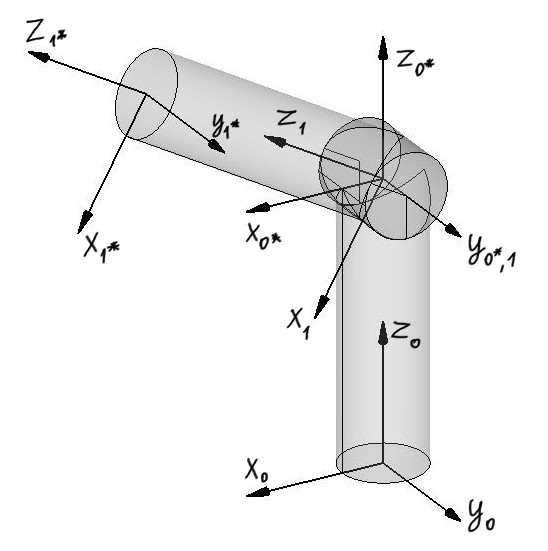
\includegraphics[width=0.6\textwidth,height=0.6\textheight,keepaspectratio]{ax3view.jpg}
  \captionof{figure}{Взаимное расположение систем координат.}
  \label{}
\end{center}

Таким образом кинематическая цепь определяется цепочкой локальных систем координат, положение каждой из которых определяется положением предыдущей и объектом трансформации СК, либо константным, либо завищим от соответствующего кинематического параметра.

Пронумеруем звенья и системы координат. Пусть неподвижное кинематическое звено, жестко связанное с лабораторной системой координат считается 0-ым, лабораторная система координат считается 0-ой СК, пусть входная система каждого $n$-ого звена считается $n$-ой СК. Выходную систему кинематического звена обозначим как $n^*$. 

Если в нашей цепи $m$ звеньев, то СК выходного звена цепи будет $m$-ой системой координат. (рассматривать $m^*$ для выходного звена цепи не имеет особого смысла).

\newpage
\section{Геометрические преобразования. Тензор положения. Тензор скорости.}

Остановимся подробнее на введенном в рассмотрение операторе трансформации систем координат. Этот оператор является тензором гомогенного преобразования, математическое представление которого может быть различным. В частности, для него могут применяться матрицы размерностью 4x4, бикватернионы, комбинация кватерниона поворота и вектора трансляции и т.д. В рамках рассматриваемого метода конкретная форма представления данного оператора взаимозаменяема и определяется исключительно удобством реализации в вычислительной системе. Обозначим этот оператор $H_{ij}$.

Введем в рассмотрение тензор положения СК. Обозначим его P. Тензор положения удобно задавать тем же набором компонент, что и тензор преобразования координат. В такой нотации компонентное выражение тензора положения $P$ j-ой системы координат взятого в i-том базисе, будет совпадать с компонентным выражением тензора преобразования СК, из базиза i-той СК в базис связанный с j-ой СК. 

\begin{equation}
P_j^{(i)} = H_{ij}^{(i)}
\end{equation}

Также введем в рассмотрение производную тензора положения j-ой системы координат

\begin{equation}\label{speed_eq} 
V_j(t) = P_j'(t) 
\end{equation}

Как и тензор преобразования системы координат и тензор положения, производная тензора положения является геометрическим объектом и имеет смысл скорости изменения геометрического положения объекта или системы координат. Часто в качестве компонентного представления производной тензора представления выбирают производные компонент тензора положения, однако такой подход не является интуитивным и не очень удобен в вычислительной реализации. В настоящем методе в качестве компонентного представления производной тензора положения выбирается пара векторов его линейной и угловой скорости $(v,\omega)$

\begin{equation}\label{speed_eq_comp} 
V_j(t) = P_j'(t) = (v_j(t),\omega_j(t)) 
\end{equation}

Такое представление не являясь явно обусловленным аналитически, удобно, в рамках метода, с вычислительной точки зрения. Использование такой системы компонентного представления приводит к тому, что уравнение (\ref{speed_eq}) не может быть в общем случае записано в компонентной форме.

Одной из возможных форм компонентного представления тензора положения является пара радиус-вектора и вектора поворота $(r,\rho)$ (порядок преобразований - сначала поворот, затем трансляция). Отметим, что, если на 6-вектор производной положения $(v,\omega)$ наложить условие колинеарности 6-вектору положения $(r,\rho)$, задача может быть сведена к одномерной, дифференциальные уравнения становятся линейными, а композиции преобразований по этой 6-оси образуют группу. В форме 3-векторов для этого должны выполняться соотношения.

\begin{equation}\label{} 
\bar{v} \upuparrows \bar{r}, \  \bar{\omega} \upuparrows \bar{\rho}, \  \frac{|\bar{v}|}{|\bar{r}|} = \frac{|\bar{\omega}|}{|\bar{\rho}|} 
\end{equation}

%\begin{figure}
%\centering
%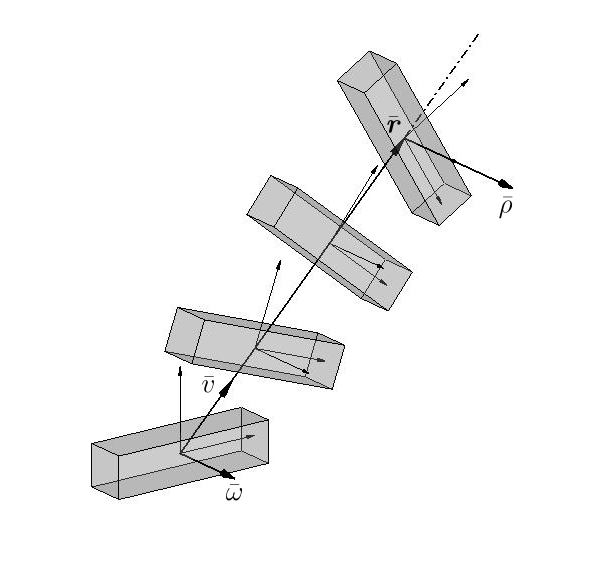
\includegraphics[width=0.8\textwidth,height=0.8\textheight,keepaspectratio]{oneaxis.png}
%\caption{Зависимость сигнала от шума для данных.}
%\label{ris:image}
%\end{figure}

\begin{center}
  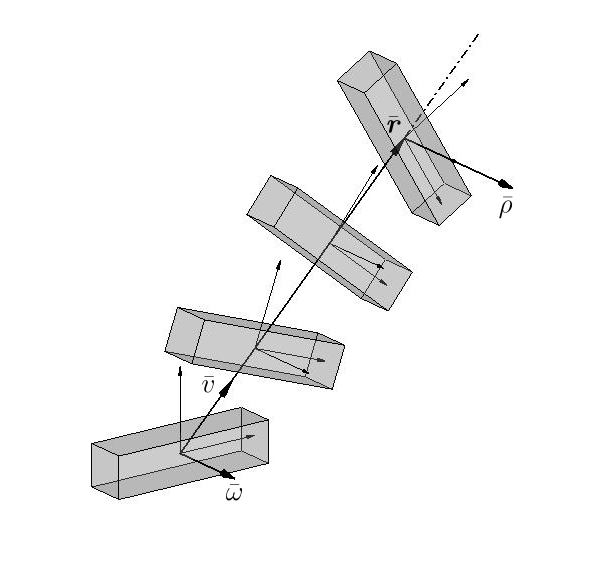
\includegraphics[width=0.8\textwidth,height=0.8\textheight,keepaspectratio]{oneaxis.png}
  \captionof{figure}{Сведение задачи к одномерному случаю.}
  \label{}
\end{center}


\begin{equation}
(\bar{v_l},\bar{\omega_l}) = (\dot{\bar{r_l}},\dot{\bar{\rho_l}})
\end{equation}

Это замечание пригодится для дальнейшего изложения.

\newpage
\section{Нахождение частных производных.}

Рассмотрим производную тензора положения $j$-ой СК в цепочке, состоящей из $n$ звеньев.
\begin{equation}\label{eq1}
V^j = \frac{dP_j}{dt} = \sum_{i=1}^{n}\frac{\partial{P_j}}{\partial{q_i}}\dot{q_i} 
\end{equation}

Поскольку от $q_i$ напрямую зависит только $P_i$, а вариации остальных $P_j, j \neq i$ являются производными,
\begin{equation}\label{}
\frac{\partial{P_j}}{\partial{q_i}} = \frac{\partial{P_j}}{\partial{P_i}}\frac{\partial{P_i}}{\partial{q_i}}
\end{equation}

Причем, очевидно, что 
\begin{equation}\label{}
\frac{\partial{P_j}}{\partial{P_i}} = 0, \ \ \forall i: i > j
\end{equation}
, поскольку эволюции последующих звеньев не могут влиять на положение предшествующих.
\begin{equation}\label{}
\frac{\partial{P_j}}{\partial{P_i}} = \frac{\partial{P_j}\partial{t}}{\partial{P_i}\partial{t}} = \frac{\partial{\dot{P}_j}}{\partial{\dot{P}_i}}
\end{equation}
\begin{equation}\label{}
\frac{\partial{P_i}}{\partial{q_i}} = \frac{\partial{P_i}\partial{t}}{\partial{q_i}\partial{t}} = \frac{\partial{\dot{P}_i}}{\partial{\dot{q}_i}}
\end{equation}

Тогда (\ref{eq1}) можно записать в тензорном виде как:
\begin{equation}\label{eq2}
V^j = \frac{\partial{\dot{P^j}}}{\partial{\dot{P}^i}}\frac{\partial{\dot{P}^i}}{\partial{\dot{q}^i}}\dot{q}^i 
\end{equation}

Переходя к записи в интересующих нас компонентах скоростей имеем:
\begin{equation}\label{matrix_spd_eq}
\begin{vmatrix}
\omega^j\\
v^j
\end{vmatrix}
=
\begin{vmatrix}
\frac{\partial{\omega^j}}{\partial{\omega^i}} & \frac{\partial{\omega^j}}{\partial{v^i}} \\
\frac{\partial{v^j}}{\partial{\omega^i}} & \frac{\partial{v^j}}{\partial{v^i}}
\end{vmatrix}
\begin{vmatrix}
\frac{\partial{\omega^i}}{\partial{\dot{q}^i}}\\
\frac{\partial{v^i}}{\partial{\dot{q}^i}}
\end{vmatrix}
\dot{q}^i
\end{equation}

В этом выражении $\omega^i$ и $v^i$ - скоростные параметры $i$-ой ЛСК. Выражение (\ref{matrix_spd_eq}) позволяет зная обобщенные скорости определить скорости всех звеньев цепи. 

До этих пор все вычисления велись в тензорном виде. Разложим вектора по базисам и проанализируем уравнения.
\begin{equation}\label{}
V^{(s)}j = H^s_i\frac{\partial{\dot{P^j}}}{\partial{\dot{P}^i}}^{(i)}\frac{\partial{\dot{P}^i}}{\partial{\dot{q}^i}}^{(i)}\dot{q}^i=H^s_jH^j_i\frac{\partial{\dot{P^j}}}{\partial{\dot{P}^i}}^{(i)}\frac{\partial{\dot{P}^i}}{\partial{\dot{q}^i}}^{(i)}\dot{q}^i
\end{equation}

Выражение 
\begin{equation}\label{}
\frac{\partial{\dot{P}^i}}{\partial{\dot{q}^i}}^{(i)}
=
\begin{vmatrix}
\frac{\partial{\omega^i}}{\partial{\dot{q}^i}}\\
\frac{\partial{v^i}}{\partial{\dot{q}^i}}
\end{vmatrix}^{(i)}
\end{equation},
разложенное по собственному базису для большого количества реальных кинематических звеньев не зависит от кинематических параметров (хотя в общем случае это не так). Так, например, для поворотного звена этот оператор равен 
\begin{equation}\label{}
W_{rot,i}^{(i)} = |s[a_x a_y a_z], [0, 0, 0]|^{T(i)}
\end{equation}, где $\bar{a}$ - орт оси вращения в связанной системе координат, а $s$ - маштабный коэффициент. Для линейного кинематического звена оператор имеет вид 
\begin{equation}\label{}
W_{act,i}^{(i)} = |[0, 0, 0], s[a_x a_y a_z]|^{T(i)}
\end{equation}, где $\bar{a}$ - орт оси трансляции в связанной системе координат, а $s$ - маштабный коэффициент. 
В этих двух наиболее часто встречающихся случаях $W_i$ является константой и может быть определён один раз, на первой итерации алгоритма.

В свою очередь выражение
\begin{equation}\label{}
\frac{\partial{\dot{P^j}}}{\partial{\dot{P}^i}}^{(i)}
=
\begin{vmatrix}
\frac{\partial{\omega^j}}{\partial{\omega^i}} & \frac{\partial{\omega^j}}{\partial{v^i}} \\
\frac{\partial{v^j}}{\partial{\omega^i}} & \frac{\partial{v^j}}{\partial{v^i}}
\end{vmatrix}^{(i)}
\end{equation}
в базисе $i$ принимает вид преобразования переноса пары векторов линейной и угловой скорости к новой точке приложения:
\begin{equation}\label{}
|\omega_j, v_j|^{T(i)} = |\omega_i,\ \omega_i \times \bar{r} + v_i|^{T(i)} = R^{(i)j}_{i}|\omega_i, v_i|^T=
\begin{vmatrix}
E & 0\\
\begin{vmatrix}
0 & r_3 & -r_2\\
-r_3 & 0 & r_1\\
r_2 & -r_1 & 0
\end{vmatrix}
^{(i)} & E
\end{vmatrix}
\begin{vmatrix}
\omega^i\\
v^i
\end{vmatrix}^{(i)}
\end{equation}, где $\bar{r}$ - вектор трансляции, связывающий центры $P_i$ и $P_j$.


%Выражение (\ref{eq2}) является решением прямой скоростной задачи кинематики в тензорном виде.
%
%Введём операторы:
%\begin{equation}\label{}
%R_i^j = \frac{\partial{\dot{P_j}}}{\partial{\dot{P_i}}}*, \ W_i = \frac{\partial{\dot{P_i}}}{\partial{\dot{q_i%}}}*
%\end{equation}
%
%\begin{equation}\label{eq2_op}
%V_n = \sum_{i=1}^{n} R_i^n(W_i(\dot{q_i})) 
%\end{equation}

%Перейдём к компонентной записи в интересующих нас базисах, используя ранее введенную компонентную форму %записи тензора скорости (\ref{speed_eq_comp}). В базисе собственной i-ой СК оператор $W_i$ имеет тривиальное %представление, обусловленное исключительно геометрией кинематического звена. Для большого количества реальных %кинематических звеньев этот оператор не зависит от кинематических параметров и записывается тривиально (хотя %в общем случае это не так). Так, например, для поворотного звена этот оператор равен 
%\begin{equation}\label{}
%W_{rot,i}^{(i)} = (s[a_x a_y a_z], [0, 0, 0])^{(i)}*
%\end{equation}, где $\bar{a}$ - орт оси вращения в связанной системе координат, а $s$ - маштабный %коэффициент. Для линейного кинематического звена оператор имеет вид 
%\begin{equation}\label{}
%W_{act,i}^{(i)} = ([0, 0, 0], s[a_x a_y a_z])^{(i)}*
%\end{equation}, где $\bar{a}$ - орт оси трансляции в связанной системе координат, а $s$ - маштабный коэффициент. 


Тогда (\ref{eq2_op}) в компонентной форме примет вид:
\begin{equation}\label{compspd1}
(\omega_n, v_n)^{(j)} = \sum_{i=1}^{n} H_i^j R_{ni}^{(i)}(W_i^{(i)}(\dot{q_i})) = \sum_{i=1}^{n} H_i^j R_{ni}^{(i)}(W_i^{(i)}([1]))\dot{q_i}
\end{equation}или
\begin{equation}\label{compspd2}
(\omega_n, v_n)^{(j)} = H^j_n \sum_{i=1}^{n} H_i^n R_{ni}^{(i)}(W_i^{(i)}([1]))\dot{q_i}
\end{equation}

В выражениях (\ref{compspd1}) и (\ref{compspd2}) $n$ - СК, для которой мы строим матрицу Якоби по набору кинематических координат $i$, $(j)$ - базис той СК, в координатах которой матрица Якоби будет выражена. Скалярная компонента $|\dot{q_i}|$ может быть вынесена в силу линейности операторов R и W. [1] - матрица размерности $1\times1$.

Запись выражения (\ref{compspd2}) через матрицу Якоби (взятую по скоростям):
\begin{equation}\label{}
J(q) = 
\end{equation}
\begin{equation}\label{}
V_n = J(q) \dot{q}
\end{equation}
\begin{equation}\label{}
(\omega_n, v_n)^{(j)} = H^{j}_{n} J^{(n)}(q) \dot{q}
\end{equation}

Алгоритм поиска скоростной матрицы Якоби для $n$-ой СК в $j$-ом базисе может выглядеть следующим образом:

1. На основе текущих координат $q_i$ вычислить трансформации $H^n_i$.
	- либо как композицию обратных преобразований,
	- либо как отношение абсолютных положений в некоторой СК. 
2. Вычислить $R(r, W_i(\bar{q},[1]))$, где r - вектор трансляции $H^n_i$.
3. Перевести полученные 6-вектора в вычислительный базис $j$. Это может быть 
	- собственный базис звена $n = j$
	- лабораторный базис $j = 0$
	- или любой другой базис $j != n,\ j != 0$


%Для вычисления компонентного представления (\ref{speed_eq_comp}), учитывая (\ref{eq1.5}), выражение (\ref{eq1}) может быть записано:

%\begin{equation}\label{eq2}
%(v_n,\omega_n) = \sum_{i=1}^{n} \frac{\partial{\dot{P_n}}}{\partial{\dot{q_i}}}\dot{q_i} = \sum_{i=1}^{n} \frac{\partial{\dot{P_n}}}{\partial{\dot{P_i}}}\frac{\partial{\dot{P_i}}}{\partial{\dot{q_i}}}\dot{q_i} 
%\end{equation}

%Или через матрицу Якоби, взятую для скоростных параметров $(v,\omega)$:
%\begin{equation}\label{eq2.5}
%(v_n,\omega_n) = J_{\dot{q_i}}^{v,\omega}\dot{q_i},\ \ i = 1 ... n
%\end{equation}





\newpage
В силу линейности координатных преобразований. 
ddP\_s / dd q\_n = ddP\_s' / dd q\_n'

 = sum( dd P\_s` / dd P\_n` * dd P\_n` / dd q\_n` * q\_n' )

 Представим тензор P\_n' в векторной форме как пару тензоров (v,w), определяющих линейную и угловую скорости соответствующей СК. При этом выражение 
 dd P\_s` / dd P\_n` примет форму оператора, вычисляющего состовляющую скоростей (v\_s, w\_s), вызванных (v\_n, w\_n). Обозначим этот оператор как R\_s\_n.

(v\_s, w\_s) = sum(  R\_s\_n * dd (v\_n,w\_n) / dd q\_n' * q\_n' )

Заметим, что в базисе n выражение dd (v\_n,w\_n) / dd q\_n' является константой и зависит от геометрии конкретного кинематического звена. Обозначим величину (dd (v\_n,w\_n) / dd q\_n')(n) как W\_n.

Запишем уравнение (* ) в базисе СК x.
(v\_s, w\_s)(x) = sum( H\_x\_n * R\_s\_n(n) * W\_n * q\_n' )
(v\_s, w\_s)(x) = H\_x\_s(x) * sum( H\_s\_n(s) * R\_s\_n(n) * W\_n * q\_n' )
(v\_s, w\_s)(s) = sum( H\_s\_n(s) * R\_s\_n(qn+1..s)(n) * W\_n * q\_n' )


Здесь H\_x\_n - это оператор гомогенного преобразования базиса n в базис x. Для векторных величин (v,w) такое преобразование означает применение вращения без трансляции.

Выражение (* ) является основным соотношением рассматриваемого метода.

Физический смысл его таков: Чтобы 

Обозначим H(i,j) - линейный оператор преобразования j-ой системы координат в i-ую. 

В текущей работе предлагается метод практической реализации алгоритма управления таким изделием.

Таким образом скорость n-ого звена в декартовой системе координат определяется суммой вкладов обобщенных скоростей кинематических коодинат. Вклад конкретной обобщенной скорости явяляется функцией этой скорости и промежуточных обобщенных координат СК (qn', qn+1 ... qs).

Выведенное соотношение соответствует прямой задаче кинематики системы, записанному в дифференциальной форме.

Выражение (* ) можно переписать в виде:
(v\_s, w\_s)(s) = sum( W\_n(q\_n ... q\_s) * k\_n ). Здесь W\_n - имеет смысл 6-вектора компоненты скорости, а k\_n - некий скалярный множитель. Таким образом (v\_s, w\_s) является линейной комбинацией векторов W\_n(q\_n ... q\_s).

Зададимся целью найти набор коэффициентов, соответствующих заданной 6-скорости (v\_s, w\_s). В общем виде задача может иметь одно решение, множество решений или не иметь решений вообще. Можно, однако утверждать, что, если заданный вектор скорости геометрически осмыслен, то задача будет иметь не менее одного решения.

В матричной форме уравнение (* ) может быть записано как:
(v\_s, w\_s) = A * K = (......)

Это уравнение может быть решено методом поиска псевдообратной матрицы, или каким-либо методом линейного программирования. Поскольку задача имеет множество решений, оптимизируемый функционал может быть введен и использован для выбора конкретного решения.

Построение следящей системы. 

На основе соотношения (* ) может быть построена следящая система положения выходного (или любого другого) звена. Для этого следует ввести положение уставки U. Тогда ошибка E системы от текущего положения P будет иметь вид:
E = U * P**-1. 

Выбрав базис (рекомендуется работа в базисе непосредственно связанном с контролируемым звеном), переведем E в 6-вектор (r, rho), где r - вектор трансляции, а rho - вектор поворота. Используем соотношение (* ) вычислим набор компонент k\_i, такой что (v\_s, w\_s) будет коллинеарным (r, rho). Вектор k\_i определен с точностью до множителя. Длина вектора может быть выбрана из физических характеристик системы и условий наложенных на управление. В простейшем случае длина вектора k\_i может линейно зависеть от длины 6-вектора (r\_s, rho\_s), что будет соответствовать апереодическому процессу регулирования.   

Построение массива точек для прохода по алгоритму линейной интерполяции. 

Соотношение (* ) может быть применено для построения массива векторов q\_i, соответствующих выполнению траектории P\_s(t). Для этого следует дискретизировать траекторию P\_s(t\_i) по массиву 0 < t\_i < t. Дискрет может быть выбран из соображений точности траектории и возможностей вычислителя.

Пусть D - тензор перехода между двумя соседними положениями.
D\_s\_s+1 = P\_s+1(q\_i) * P\_s(q\_j)**-1

Вычислим D как 6-вектор (r, rho). Итеративно вычисляя компоненты k\_i для текущего модельного положения используем виртуальную следящую систему, переместим виртуальную модельную систему из положения P\_s в положение P\_s+1. Геометрически это соответствует численному вычислению минимума функции E(q\_i) = U * P**-1, методом градиентного спуска. Так как кинематические уравнения в общем случае нелинейны, метод может иметь недостатончно хорошую сходимость. Сходимость метода тем лучше, чем плотнее взят набор точек P\_s(t\_i).  



\end{document}

